\begin{figure}[h]
  \centering
  %Define block styles
  \tikzstyle{decision} = [diamond, draw, fill=blue!20, 
  text width=4.5em, text badly centered, node distance=3cm, inner sep=0pt]
  \tikzstyle{block} = [rectangle, draw, fill=blue!20, text width=12em, text
  centered, rounded corners, minimum height=3em]
  \tikzstyle{line} = [draw, -latex']
  \tikzstyle{cloud} = [draw, ellipse,fill=red!20, node distance=3cm, minimum
  height=2em]
  
    
  \begin{tikzpicture}[node distance = 2cm, auto]
    % Place nodes
    \node [cloud] (xAOD)  {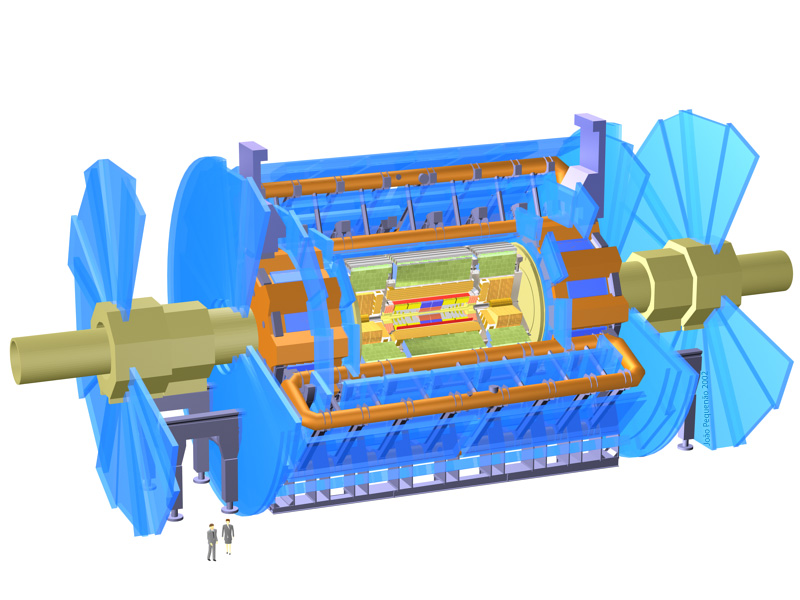
\includegraphics[width=.25\textwidth]{atlas_big}};;
    
    \node[cloud, left=3cm of xAOD] (DxAOD) {DxAOD};
    \node[left=1.5cm of xAOD] (ghost) {};

    \node[block, below=1.5cm of ghost] (CxAODMaker) {CxAOD Maker};
    \node[cloud, below=1.5cm of CxAODMaker] (CxAOD) {CxAOD};

    \node[block, below=1.5cm of CxAOD] (CxAODReader) {CxAOD Reader};
    \node[below=1.5cm of CxAODReader] (ghost2) {};

    \node[cloud, left=1.5cm of ghost2] (nTuple) {nTuple};
    \node[cloud, right=1.5cm of ghost2] (hist) {Histograms};

    \node[block, below=1.5cm of hist] (fit) {Fitting Framework};
    \node[block, below=1.5cm of nTuple] (rd) {Research \& Development};
    
    % Draw edges 
    \path [line] (xAOD) -- (CxAODMaker);
    \path [line] (DxAOD) -- (CxAODMaker);
    
    \path [line] (CxAODMaker) -- (CxAOD);
    \path [line] (CxAOD) -- (CxAODReader);

    \path [line] (CxAODReader) -- (nTuple);
    \path [line] (CxAODReader) -- (hist);

    \path [line] (hist) -- (fit);
    \path [line] (nTuple) -- (rd);
  \end{tikzpicture}
  \caption{A flow chart showing the CxAOD Framework data processing chain. The
    red elliptical nodes indicate data formats and the blue rectangular nodes
    indicate software modules.}
  \label{fig:cxaod-flow}
\end{figure}
